\documentclass[times, utf8,projekt]{fer}
\usepackage{booktabs}
\usepackage{amsmath}
\usepackage{hyperref}
\usepackage{titlesec}
\usepackage{graphicx}
\usepackage{xurl}
\usepackage{natbib}
\usepackage{color}
\usepackage[nodayofweek,level]{datetime}
%\usepackage[numbers,square]{natbib}
\usepackage{etoolbox}
\makeatletter
\patchcmd{\chapter}{\if@openright\cleardoublepage\else\clearpage\fi}{}{}{}
\makeatother
\setcitestyle{numbers}
\usepackage{standalone}
\graphicspath{{figures/}}
\PassOptionsToPackage{hyphens}{url}\usepackage{hyperref}

\begin{document}
	
	% TODO: Navedite broj rada.
	%\thesisnumber{000}
	
	% TODO: Navedite naslov rada.
	\title{Umjetna inteligencija u adaptivnom učenju}
	
	% TODO: Navedite vaše ime i prezime.
	\author{Jelena Nemčić, Marin Ovčariček,Zvonimir Sučić,Ivana Žeger}
	
	\maketitle
	% stranice s napomenom o umetanju izvornika rada. Uklonite naredbu \izvornik ako želite izbaciti tu stranicu.
	%\izvornik
	% Dodavanje zahvale ili prazne stranice. Ako ne želite dodati zahvalu, naredbu ostavite radi prazne stranice.
	%\zahvala{}
	\tableofcontents
\chapter{Uvod}
Adaptivno učenje u e-learning softverima tipično funkcionira tako da mjeri razinu znanja korisnika kroz početni skup pitanja, virtualnu simulaciju i/ili dodijeljene zadatke. Na temelju podataka prikupljenih iz odgovora korisnika, takav softver u stvarnom vremenu procjenjuje razliku između korisničkog znanja i znanja potrebnih za određenu kompetenciju, te odabire lekcije i zadatke za korisnika tako da minimizira količinu edukacijskog sadržaja koji tom korisniku prikazuje.\newline
Konstrukcija algoritma za određivanje puta za adaptivno učenje tipično se radi na dva načina: 1) kreiranjem formalnog modela znanja za određenu domenu, a koji kreiraju eksperti iz te domene ili 2) koristeći algoritamski pristup baziran na teorijama Bayesian Knowledge Tracing i Item Response Theory koji na temelju odgovora polaznika edukacije procjenjuje vjerojatnost da je polaznik usvojio određenu vještinu/koncept (što ponovno zahtijeva unaprijed definirane vještine/koncepte).\newline
U posljednje vrijeme, a s obzirom na dostupnost sve većih količina podataka (big data) ponovno su oživjele i dodatno se razvijaju tehnologije kreiranja grafova znanja (npr. pomoću dubokog učenja), a koji s obzirom na to da su kreirani statistički mogu biti mnogo kompleksniji i uže segmentirani (precizniji) u odnosu na one koje kreiraju eksperti nekog područja. Dodatno, prikupljanje velike količine informacija u različitim domenama omogućuje da kreiranje grafova znanja ne bude ograničeno samo na one tvrtke koje imaju golem broj korisnika kao što su Google ili Facebook). Na temelju inicijalnog istraživanja vjerujemo da se ova metoda može primijeniti i na kreiranje grafova znanja za adaptivno učenje, te time omogućiti s jedne strane znatno veću adaptivnost, a s druge strane veću jednostavnost kreiranja takvih grafova.\newline
Ovo je posebno važno za područja edukacije izvan formalnog obrazovanja, gdje nisu strogo definirane ishodi učenja i testovi kojima se mjeri je li neki ishod učenja dostignut kod pojedinog polaznika. Dva primjera za to su instrukcije, gdje učeniku često nedostaju i predznanja iz drugih područja koje je ranije u školi trebao usvojiti, te korporativne edukacije, koje često obuhvaćaju ljude različitih struka i različitim znanjima iz domene za koju nastoje dobiti certifikat.


\chapter{Cilj i postupak}
Stoga je cilj ovog projekta provjeriti sljedeće:
\begin{itemize}
\item Provjera mogućnosti kreiranja grafa znanja isključivo na temelju točnosti odgovora na zadacima iz jedne domene znanja koje korisnici daju i informacije o redoslijedu zadavanja zadataka pojedinom korisniku
\item Ako je navedeno moguće, potrebno je provjeriti može li se kreirati graf znanja na temelju rješavanja zadataka za istu domenu na temelju parcijalnog broja zadataka (što realnije reprezentira dostupne zadatke za stvarne domene – rijetko su dostupna baš sva znanja iz neke domene da bi se mogla kreirati zadaci koji pokrivaju baš svaku informaciju u toj domeni)
\item Ako je navedeno moguće, potrebno je provjeriti može li se isto napraviti i za neku domenu realnog znanja\newline
\end{itemize}
Ukratko, ovim se projektom provjerava može li se graf znanja potreban za adaptivno učenje kreirati metodama dubokog učenja na temelju ponašanja korisnika na zadacima (probabilistički), a bez potrebe za time da eksperti unaprijed određuju koncepte/vještine u koje se grupiraju zadaci ili čak sam graf znanja.\newline\newline
Za potrebe ove provjere kreirat će se:
\begin{itemize}
	\item umjetni, zatvoreni graf znanja 
	\item zadaci koji pokrivaju sve informacije prisutne u tom zatvorenom grafu znanja\newline
\end{itemize}
Potom će se zadaci dati testerima na rješavanje, tako da se:
\begin{itemize}
	\item varira redoslijed zadataka koje pojedini tester dobiva kako bi pokrio sve kombinacije
	\item bilježi točnost odgovora testera na zadatak
	\item u slučaju netočnog odgovora testeru se prikazuje točna informacija.
\end{itemize}

\chapter{Postojeće ideje i koncepti}
Istraživanjem fraza kao što su Bayesian Knowledge Tracing (BKT), Item Response Theory (IRT), Deep Knowledge Tracing (DKT), Intelligent Tutoring Systems (ITS), Massive Open Online Courses (MOOC), itd. pronađeni su mnogi radovi koji su služili kao sredstvo upoznavanja s tematikom rada i inpiracija za daljnja ostvarenja. 
\newline
\newline
Među prvima pronađena je i proučena platforma adaptivnog učenja Knewton korištena za personalizaciju edukacijskog sadržaja \citep{knewton}. 
\newline
\newline
Izazovnim područjem praćenja znanja (engl. \textit{knowledge tracing}) moguće je strojno modelirati znanje korisnika pomoću njegove interakcije s računalom tijekom procesa učenja \citep{dkt}. Korisnicima je predložen sadržaj učenja ovisno o njihovim potrebama (sadržaj je okarakteriziran kao prelagan, pretežak, moguće ga je potpuno preskočiti ili ostaviti za kasnije). Predviđaju se buduće korisničke performanse prema prošloj aktivnosti. Mnoge metode pri tome uključuju korištenje Markovljevih modela s ograničenom funkcionalnošću. Također, neki modeli koriste logističku regresiju uz PFA (engl. \textit{performance factors analysis}). U novije vrijeme, korištene su povratne neuronske mreže (engl. \textit{recurrent neural networks, RNN}) pa cjelokupni model nosi naziv Deep Knowledge Tracing (DKT). Posebice je popularna kompleksnija varijanta RNN-a, LSTM (engl. \textit{long short-term memory}). Interakcije (pitanje-odgovor) potrebno je pretvarati u vektore fiksne duljine (ideja je inpute predstaviti one-hot encodingom parova (oznaka zadatka, točnost)). Mapiranje u izlazne vrijednosti postiže se računom slijeda “skrivenih” stanja (uzastopnim enkodiranjem bitnih informacija proteklih zapažanja kako bi odgovarale budućim predikcijama). Izlazna vrijednost je vektor vjerojatnosti točnog rješavanja svakog od zadataka u modelu. 
Sposobnost predviđanja korisničkih performansi ispitana je na simuliranom skupu podataka. Umjetno su generirani korisnici koji rješavaju određen broj zadataka iz fiksnog skupa koncepata. Svaki korisnik ima latentnu “vještinu” za svaki koncept, a svaki zadatak ima koncept i težinu. Vjerojatnosti da korisnik točno riješi zadatak određene težine ako ima određenu vještinu modelirane su pomoću IRT-a. Također, otkriven je javno dostupan benchmark skup podataka, 2009-10 Assistments Data.
\newline
\newline
Ponađen je i proučen i sustav KnowEdu, kojem je cilj konstruirati grafove znanja za edukacijske potrebe i identificirati odnose između različitih koncepata \citep{knowedu}.\newline
Na početku se pokušavaju ustanoviti svi koncepti koji se nalaze u dostupnim nastavnim materijalima i tečajevima korištenjem strojnog učenja. Zatim se koriste CRF (engl. \textit{conditional random field}) model, povratna neuronska mreža i varijanta LSTM mreže, GRU (engl. \textit{gated recurrent units}) kako bi se dobio graf preduvjeta. Skup podataka prikupljen je iz više testova pri čemu je svaki ispitanik riješio svaki test. Jedan test sastoji se od više pitanja koja ispituju znanje istog koncepta i pomoću njega se izračuna odgovarajuća ocjena znanja tog koncepta za svakog ispitanika. Ocjene predstavljaju vještine ispitanika u tom području i one su ulaz modela. Svaki model kao izlaz daje, za svaku kombinaciju koncepata, vjerojatnost da je koncept A preduvjet za znanje koncepta B.
\documentclass{report}
\usepackage{amsmath}
\usepackage{hyperref}
\begin{document}
	\title{Bayesian knowledge tracing (BKT)}
		
	\maketitle
		
	\chapter{Uvod}
	\section{Općenito o BKT}
		Bayesian Knowledge Tracing koristi Hidden Markov Model i ima 4 osnovna parametra:
		\begin{itemize}
			\item p(L0) - vjerojatnost da je korisnik a priori savladao gradivo
			\item p(G) - vjerojatnost da je korisnik pogodio točan odgovor bez da ima potrebno znanje	
			\item p(S) - vjerojatnost da je korisnik krivo odgovorio iako ima potrebno znanje	
			\item p(T) - vjerojatnost da je znanje prešlo iz NE ZNA u ZNA nakon prilike da se primjeni znanje
		\end{itemize}
		Kao izlaz dobivaju se vrijednosti:
		\begin{itemize}
			\item p(L) - vjerojatnost ovladavanja vještinom (eng. probability of skill mastery)
			\item p(C) - vjerojatnost da će korisnik ispravno primijeniti vještinu u budućnosti (eng. probability of the student correctly applying the skill on a future practice)
		\end{itemize}
	\begin{equation}
		$p(L_t\mid obs=correct)=\frac{p(L_t)*(1-p(S))}{p(L_t)*(1-p(S)+(1-p(L_t)*p(G))}$
	\end{equation}
	\begin{equation}
		$p(L_t\mid obs=wrong)=\frac{p(L_t)*p(S)}{p(L_t)*p(S)+(1-p(L_t)*(1-p(G))}$
	\end{equation}
	\begin{equation}
	$p(L_{t+1})=p(L_t\mid obs=correct) + (1-p(L_t\mid obs=correct))*p(T)
	\end{equation}
	\begin{equation}
	$p(C_{t+1})=p(L_{t+1}) * (1-p(S)) + p(L_{t+1})*p(G)
	\end{equation}
	\section{Ideje}
		Prvobitna ideja je bila da se p(L0) računa iz inicijalnih pitanja, vrijednosti p(G) i p(S) bi se prema preporuci iz rada(trebalo bi pronaći kojeg i baciti referencu) stavile na interval [0,0.3], [0,0.1] te bi se p(T) postavio prema preporuci eksperta što ne želimo jer je cilj ovog projekta da smanjimo zadatke eksperata na minimum.
		
		To je ukazalo na potrebu pronalaska algoritama koji bi uz pomoć nekog skupa podataka aproksimirali parametre za BKT.
	\section{Problemi i zadaci}
	\begin{itemize}
		\item proučiti parametar p(T)
		\item proučiti kodove sa githuba kako bi se dobila ideja kako algoritam funkcionira
		\item napraviti malu implementaciju s malo pitanja i provjeriti radi li
		\item proučiti parameter fitting uz pomoć EM algoritma, stohastic gradient descenta ili neke druge metode
		\item kako napraviti input dataset, prikupiti podatke
		
	
	\end{itemize}
	\chapter{Dobivanje BKT parametara}
	\section{EM (expectation-maximization) algoritam}
		\begin{itemize}
			\item iterativni algoritam za pronalaženje (aproksimiranje) najveće izglednosti (eng. maximum likelihood) ili maksimalne a posteriori (MAP) procjene parametara u statističkim modelima
			\item model ovisi o nepoznatim latentnim varijablama
			\item EM iteracija sadrži 2 koraka:
				\begin{itemize}
					\item 	korak očekivanja (E), koji stvara funkciju za očekivanje log-izglednosti koja se procjenjuje pomoću trenutne procjene parametara, procjenjuju se vrijednosti latentnih varijabli
					\item 	korak maksimizacije (M), koji izračunava parametre distribucije koji maksimiziraju očekivanu log-izglednost pronađenu u E koraku, ti se parametri zatim koriste za procjenu latentnih varijabli u sljedećem E koraku
				\end{itemize}
			
			\item primjenjuje se kada želimo odrediti parametre distribucije (normalna, eksponencijalna, …)
			\item problem: za korištenje potrebo znati distribuciju podataka ili točne vrijednosti (eng. true values) traženih parametara
			
		\end{itemize}
	Kroz ovo istraživanje nije pronađena niti jedna implementacija EM algoritma za aproksimaciju BKT parametara niti je napravljena vlastiti implementacija zbog prevelikog praga znanja matematike.
	
	\section{Grid search i Simulated Annealing}
		Pronađen je kod napisan u Javi koji računa BKT parametre tehnikom simuliranog kaljenja \url{https://github.com/wlmiller/BKTSimulatedAnnealing}. U README na githubu se također spominjao kod koji je bio baza za to, on je koristio običan grid search kako bi izračunao parametre. Oba koda su prevedena u python i prilagođena našim skupovima podataka. Na kraju se ispostavilo da je "simulirano kaljenje" povoljnije te se grid search odbacio.
	\chapter{Rezultati}
		\begin{itemize}
			\item napravljen google forms kviz sa 20 pitanja iz biologije, ispitanici moraju odgovoriti na svih 20 pitanja kako bi podaci ušli u dataset
			\item napravljena python skripta koja pretvara podatke dobivene iz google formsa u oblik prikladan za treniranje BKT-a i pronalaženje parametara
			\item pronađen je kod u Javi koji tehnikom simuliranog kaljenja aproksimira parametre za BKT uz pomoć danog dataseta, kod je preveden u python skript
			\item napravljena python skripta za BKT koja određuje vjerojatnost da je ispitanik naučio/  savladao gradivo
			\item uz pomoć skripte za aproksimaciju BKT parametara, nađene su njihove vrijednosti za svaku vještinu iz ASSISTMENTS dataseta i pohranjenje u google sheets tablicu
			\item dobiveni parametri algoritmom simuliranog kaljenja uspoređeni su s onima dobivenima pomoću grid search metode -> vrijednosti parametara su skoro iste, vrlo male razlike
			\item napravljen google forms kviz sa po 6 pitanja iz 5 koncepata, izračunati su parametri za taj dataset
			\item BKT kod i kod za aproksimaciju BKT parametara su se dalje koristili u bilježnicama za izgradnju grafa probabilističkim metodama
			
		\end{itemize}
	\chapter{Poveznice}
	\section{BKT}
	\url{https://en.wikipedia.org/wiki/Bayesian_Knowledge_Tracing}\newline
	\url{http://www.cs.cmu.edu/~./ggordon/yudelson-koedinger-gordon-individualized-bayesian-knowledge-tracing.pdf}\newline
	\url{https://github.com/CAHLR/pyBKT/blob/master/README.md}\newline
	\url{https://www.learnlab.org/uploads/mypslc/publications/bca2008v.pdf}\newline
	\url{https://www.upenn.edu/learninganalytics/ryanbaker/paper_143.pdf}\newline
	\url{https://github.com/yemao616/Bayesian-Knowledge-Tracing}\newline
	\url{http://www.cs.cmu.edu/~./ggordon/yudelson-koedinger-gordon-individualized-bayesian-knowledge-tracing.pdf}\newline
	\url{https://www.fi.muni.cz/~xpelanek/publications/umuai-overview.pdf}\newline
	\url{https://medium.com/@joyboseroy/modelling-a-students-learning-34375b0131dd}\newline
	\url{https://www.math.vu.nl/~sbhulai/publications/data_analytics2018c.pdf}\newline
	\section{Pronalaženje parametara}
	\url{https://www.fmrib.ox.ac.uk/datasets/techrep/tr00yz1/tr00yz1/node9.html}\newline
	\url{https://github.com/wlmiller/BKTSimulatedAnnealing/blob/master/computeKTparams_SA.java}\newline
	\url{https://www.upenn.edu/learninganalytics/ryanbaker/paper_143.pdf}\newline
	\url{https://educationaldatamining.org/files/conferences/EDM2018/papers/EDM2018_paper_14.pdf}\newline
	\url{http://yudelson.info/hmm-scalable/}\newline
	\url{https://www.educationaldatamining.org/EDM2015/proceedings/short364-367.pdf}\newline
	\url{https://concord.org/wp-content/uploads/2016/12/pdf/tracking-student-progress-in-a-game-like-learning-environment.pdf}\newline
	\url{https://tinyheero.github.io/2016/01/03/gmm-em.html}\newline
	\url{https://machinelearningmastery.com/expectation-maximization-em-algorithm/}\newline
	\url{http://rstudio-pubs-static.s3.amazonaws.com/1001_3177e85f5e4840be840c84452780db52.html}\newline
	\url{https://www.colorado.edu/amath/sites/default/files/attached-files/em_algorithm.pdf}
\end{document}
\chapter{Bayes graf}
	\section{Uvod}
	
	Ideja je napraviti vlastiti model koji iz skupa podataka računa vjerojatnost savladavanja koncepata te se prema njima gradi graf znanja.\newline
	Prvi pristup je račun uvjetnih vjerojatnosti $p(Y_j\mid X_i)$, odnosno vjerojatnost da korisnik zna (savladao je) koncept Y ako zna X. Koristi se klasična formula Bayesove uvjetne vjerojatnosti čime se gradi matrica odnosa koncepata.
	\begin{equation}
		p(Y \mid X)=\frac{p(X \wedge Y)}{p(X)}
	\end{equation}
	\newline Vjerojatnost Y uz X nam govori koliko je poznavanje X bitno za poznavanje Y. Pretpostavka je da će korisnik s većom vjerojatnošću znati jednostavniji koncept ako zna kompliciraniji (nadogradnju jednostavnog), ako su X uz Y i Y uz X podjednaki (potreban je neki prag) može se pretpostaviti da su koncepti nezavisni ili bi se mogli spojiti kao jedan koncept. \newline
	Drugi pristup je bio pokušaj da se gleda kad su koncepti X i Y točni s obzirom koji od njih je položen prvi, pretpostavka je bila da bi se tako mogla odrediti relacija nadogradnje, odnosno prethodnika. Pristup nije uspio jer ili nije moguć ili nije bio dobro definiran / implementiran.\newline
	Najveći problem u oba pristupa je to što pokušavamo dobiti ovisnosti među konceptima,a ne pitanjima. Za razliku od pitanja za koncepte se ne može reći da ih se zna/ne zna jer se oni sastoje od više pitanja te se može samo gledati postotak riješenosti za svakog studenta / prosječan postotak riješenosti. Prosječan postotak rješenosti se može gledati kao pripadnost neizrazitom skupu ZNA odnosno 1- postotak riješenosti kao pripadnost skupu NE ZNA, to komplicira stvari kod Bayesovog zaključka. Potrebno je pronaći/proučiti postoji li ekvivalent Bayesovog zaključka kada se koriste neizraziti skupovi odnosno kontinuirane vrijednosti [0,1].\newline
	Ideja:
	\begin{itemize}
		\item iz dataseta izračunati parametre BKT-a algoritmom po izboru
		\item uz pomoć BKT-a odrediti je li neki student savladao gradivo na temelju odgovora na pitanja (vratiti se u diskretno područje)
		\item na temelju tih rezultata raditi matricu uvjetnih vjerojatnosti\newline
	\end{itemize}
	Problemi:
	\begin{itemize}
		\item Je li dobro korisiti isti dataset za aproksimaciju BKT parametara i onda nad tim istim datasetom uz pomoć BKT-a određivati je li neki student savladao određeno gradivo?
		\item 	Koliko bi trebali biti veliki datasetovi za aproksimaciju i izgradnju grafa kako bi se dobili neki smisleni rezultati?\newline
	\end{itemize}
	Pretpostavke:
	\begin{itemize}
		\item svi studenti odgovaraju na sva pitanja iz svih koncepata
		\item svi studenti moraju istim redoslijedom odgovarati na pitanja
		\item budući da se koriste metode s vjerojatnostima (Bayes) potrebna je veća količina podataka kako bi rezultati imali smisla
	\end{itemize}

	\section{Problem kontinuiranih vrijednosti}
		Običan Bayesov zaključan radi sa diskretnih vrijednostima (true/false, 1/0). Dok je to istina kod izračuna vjerojatnosti i točnosti pitanja, isto se ne može reći za koncepte. Može se gledati da je koncept položen s nekom vjerojatnošću ili da određen pokušaj ispita pripada skupo "položen" s nekom pripadnošću, to je obično postotak točnih bodova i to je racionalan broj. Iako postoji Bayesov zaključak za kontinuirane vrijednosti nije jednostavan za izračunati jer se teško mogu dobiti latentne razdiobe bodova za neku populaciju. Pošto je Bayes kontinuiranoj domeni prekompliciran za računati potražena je altrenativa te se došlo do zaključka da se treba nekako vratiti u diskretnu domenu, odnosno napraviti model koji može odlučiti kad neki koncept je ili nije položen.\newline
		Najjednostavnije rješenje je ručno za svaki koncept zadati bodovni prag te bi svi korisnici koji zadovolje prag imali oznaku da su savladali koncept. To i nije najbolji pristup jer se ne uzimaju u obzir razne druge varijable kao što su npr. vjerojatnost da korisnik pogađa ili slučajno pogrješi.\newline
		Kako bi se rješio taj problem, pronađena je tehnika Bayesian Knowledge Tracing~\ref{ch:BKT} i kombinirana sa vlastitom tehnikom raspodjele po Gaussu kako bi se bolje aproksimiralo trenutno znanje korisnika.
	\section{Skaliranje korisnika prema Gaussu}
		Kao alternativa BKT-u implementirano je skaliranje studenata prema Gaussu:
	\begin{itemize}
		\item za svakog studenta i za svaku vještinu izračunat je percentil kojemu taj student pripada u ovisnosti o odgovorima svih studenata
		\item postavi se threshold koji odgovara percentilu iznad kojeg se nalaze studenti koji su položili vještinu\newline
	\end{itemize}
		Paralelno se za svakog studenta računa prolaznost (0 ili 1) prema BKT-u i prema Gaussu:
	\begin{itemize}
		\item ako se one poklapaju, to se uzima kao vrijednost za tog studenta
		\item ako je zbroj te dvije jačine veći od 0, uzima se da je student položio vještinu
		\item ako su različite gleda se jačina s kojom model tvrdi da je student pao/položio, ona se računa na sljedeći način:
	\end{itemize}
	\begin{figure}[!htb]
		\centering
		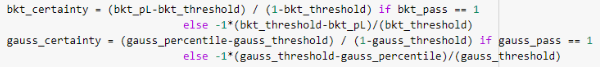
\includegraphics[scale=1]{Bayes_kod.png}
		\caption{}
		\label{}
	\end{figure}
		
	\section{Izvještaji}
		\subsection{22.07.2020.}
		\textbf{Planovi, problemi:}
		\begin{itemize}
			\item pronaći dobru vrijednost za cutoff kod micanja poveznica kod grafa
			\item iteriranje po retcima dataframeova - nije dobro, treba pronaći efikasnije načine obrade tablica
			\item isprobati program na malom datasetu
			\item isprobati program na biologija dataset, ali gledajući da je svako pitanje jedan koncept (napraviti i program koji bi pretvorio pitanja u koncepte)
			\item proučiti librarye za crtanje usmjerenih grafova (boje, labele, debljine poveznica)
			\item dopuniti program da crta usmjerene grafove
			\item pokušati naći implementacije EM i grid search algoritma za računanje BKT parametara
			\item pokušati pronaći dobro objašnjenog bayesa u kontinuiranoj domeni
			\item pronaći naprednije implementacije BKT-a koje uzimaju više parametara
			\item osmisliti strukture podataka koje bi predstavljale čvorove i povezivale pitanja,koncepte i ostale čvorove u jednu cjelinu, omogućavale obilazak grafa te nalaženje najkraćeg puta (po nekom kriteriju) od početnog do ciljnog čvora
			\item napraviti novi test koji bi imao mali broj pitanja iz različitih područja koja su međusobno povezana (npr. stanica, što je to -> građa stanice -> građa različitih organela) i na tome isprobati program\newline
		\end{itemize}
		\textbf{Rezultati}
		\begin{itemize}
			\item napravljena skripta za izgradnju grafa pomoću uvjetnih vjerojatnosti i Bayesove formule
			\begin{itemize}
				\item ulaz: datoteka koja sadrži BKT parametre za sve vještine i datoteka koja sadrži tablicu studenata i njihovih odgovora
				\item izlaz: matrica koja predstavlja matricu susjedstva grafa, gdje svaki element predstavlja “jačinu”/”vjerojatnost” s kojom je koncept \textit{i} povezan s konceptom \textit{j}
				\item skripta sadrži razred BKT i funkcije za računanje vjerojatnosti p(X), računanje zajedničke vjerojatnosti p(X and Y) i računanje matrice ovisnosti
			\end{itemize}
			\item skripta je isprobana na dosad prikupljenim podacima testa za biologiju (74 odgovora) i dobiveni su realni rezultati, ali nismo imali sa čime usporediti budući da je to samo jedan koncept
			\item izrađeni su grafovi na malom umjetnom datasetu i datasetu biologija gdje su se pitanja gledali kao zasebni koncepti
			\item za potrebu prilagodbe pitanja u koncept napravljena je skripta koja uzima pitanja kao koncepte, računa vjerojatnosti te crta graf
			\item za crtanje grafova koristio se netowrkx library
			\item vrijednost cutoffa za izgradnju grafova bi prema procjeni trebala u intervalu [0.8,0.95]. Nismo našli nikakve službene izvore/preporuke tako da  će se za sada cutoff morati ručno procijeniti.
			\item odrađena optimizacija koda gdje se boljim iteriranjem po dataframeu dobiva ljepši i brži kod, daljnja optimizacija je vjerojatno moguća, ali trenutno nije prioritet trošiti vrijeme na istraživanje kako to napraviti
		\end{itemize}
		\subsection{28.07.2020.}
		\begin{itemize}
			\item napravljen je je novi kviz sa pet koncepata iz biologije
			\item svaki koncept ima 6 pitanja
			\item problemi: kviz ima više pitanja nego prošli, u prosjeku je mentalno zahtjevniji, znanje koncepta vjerojatno nije dobro pokriveno sa tih 6 pitanja, neki koncepti su su značajno zahtjevniji nego drugi te raspodjela pitanja po težini nije ista u svakom konceptu i vjerojatno nije optimalna budući da se trenutno svi odgovori vrednuju jednako
			\item u trenutku pisanja izvještaja imamo samo 25 odgovora na kviz, pokrenuli smo model da vidimo kako reagira na manjak podataka
			\item rezultati su očekivano lošiji nego prije, u početku su od 5 koncepata na grafu bila prikazana samo 3 te smo dobili NaN vrijednosti matrici povezanosti, što se dogodilo jer prema pragu BKT-a niti jedan student nije položio predmet te se pojavilo dijeljenje sa nulom. Nakon što smo spustili prag prolaska sa 0.95 na 0.9, pojavio se dodatan čvor na grafu i nismo imali NaN, ovo ukazuje na problem osjetljivosti BKT-a na manjak podataka i na redoslijed točno/netočno odgovora studenata
			\item također same povezanosti grafa nisu imali smisla (npr. da je živčana stanica preduvjet za diobu stanice)
			\item ovi rezultati nisu iznenađujući jer je samo svojstvo BKT-a da je osjetljiv na redoslijed i uzastopno ponavljanje točno/netočno u nizu odgovora te su modeli bazirani na vjerojatnostima jako osjetljivi na manjak ulaznih podataka
			\item IDEJA: isprobati jednostavno skaliranje bodova studenata na temelju Gaussove raspodjele te odrediti prag prema kojem bi se dijelili na prolazak/pad. Ovako bi se maknula loša svojstva BKT-a, ali bi model postao još jednostavniji te bi vjerojatno imao slabija svojstva predviđanja.
			\item treba proučiti kako napraviti da linije povezanosti imaju različite debljine s obzirom na jačinu povezanosti, onda bi se mogao malo spustiti cutoff da se dobije bolji pregled ovisnosti između koncepata
		\end{itemize}
		\begin{figure}[!htb]
		\centering
		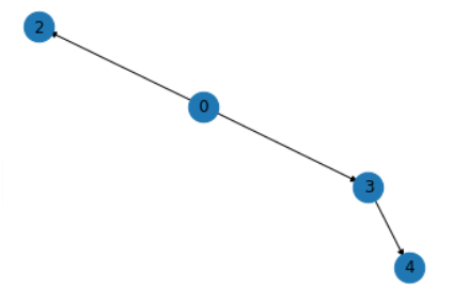
\includegraphics[scale=1]{Bayes_graf3.png}
		\caption{}
		\label{}
		\end{figure}
		Legenda:
		
		0: Stanica
		1: DNA
		2: Stanični metabolizam
		3: Dioba stanice
		4: Živčana stanica

		\subsection{29.07.2020.}
		\begin{itemize}
			\item napravljen program koji generira proizvoljan umjetan dataset
			\item obavezni ulazni argumenti su broj studenata i trojka (broj pitanja po konceptu, prosječni udio točnih odgovora u tom konceptu, standardna devijacija)
			\item skripta pretpostavlja da svaki student odgovara na sve koncepte i na sva pitanja
			\item prema gaussovoj raspodjeli svakog koncepta se svakom studentu pridjeljuje postotak točno riješenih zadataka te mu se prema toma generiranju rješenja
			\item dataset se sprema u klasičnom obliku kojeg naše skripte za crtanje mogu koristiti
			\item u trenutku pisanja ima 75 odgovora na novu anketu
			\item pokrenuta je obrada podataka i izračunavanje bkt parametara za trenutne odgovore
			\item cutoff threshold je 0.5
		\end{itemize}
		\begin{figure}[!htb]
			\centering
			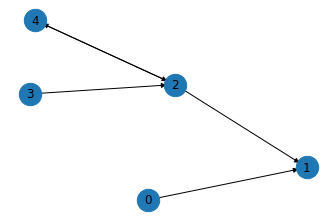
\includegraphics[scale=1]{Bayes_graf4.png}
			\caption{}
			\label{}
		\end{figure}
		Legenda:
		
		0 : Stanica
		1 : DNA
		2 : Živčana stanica
		3 : Stanični metabolizam
		4 : Dioba stanice\newline
		\newline Zaključci: ljudi koji su znali diobu stanicu i stanični metabolizem generalno su znali i živčanu stanicu, ljudi koji su znali diobu stanice obično su znali i živčanu stanicu te ljudi koji su znali DNA su obično znali i stanicu/živčanu stanicu. Ovo ne prikazuje realan slijed učenja biologije, ali nije ni očekivano da prikazuje jer biologija nema tako strogi uvjetni slijed koncepata kao npr. matematika\newline
		\newline \textbf{Rezultati umjetnih datasetova}	\newline
		BKT-annealing daje predzadnjem konceptu jako male vrijednosti parametara zbog čega nitko ne prolazi taj predmet, dobivaju se NaN vrijednosti te se ne crta taj čvor.
		\begin{figure}[!htb]
			\centering
			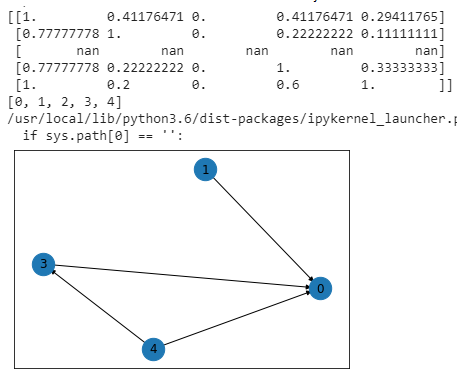
\includegraphics[scale=1]{Bayes_graf6.png}
			\caption{}
			\label{}
		\end{figure}
		Ovo ukazuje na veliku osjetljivost aproksimacije parametara na broj i redoslijed točnih odgovora studenata, ovo se može poboljšati pažljivim odabirom mean i stddev vrijednosti kod generiranja umjetnog dataseta (ne odabrati premali mean te pogotovo ne uzimati veliki stddev kod malog meana i uz mali broj studenata jer se može dogoditi da većina njih dobije male postotke riješenih zadataka što daje loše bkt parametre). Drugi način je staviti nekakvo zaglađivanje kako bi se onemogućilo dobivanje NaN vrijednosti s nekom malom konstantom (ovo samo sprječava errore, ali ne pomaže u točnosti modela). Zadnje što ostaje je pronaći i razviti alternativu BKT-u koja nije toliko osjetljiva.
		\subsection{30.07.2020.}
		\begin{itemize}
			\item 	ideja: trenutno je za model potrebno da svi studenti rješavaju sve koncepte, to nije pojava u realnim skupovima podataka pa se predlaže sljedeće rješenje - kod računa joint\_probabilitya uzeti presjek studenata koji su rješavali koncept A i koncept B po njihovom student\_id-u, sam izračun pX se ostavi kao što je i bio. Ova pretpostavka bi mogla vrijediti jer ako je realan skup podataka dovoljno velik te ako je presjek također dovoljno velik oni će imati dovoljno informacije da se da realni prikaz ovisnosti između koncepata
			\item ideja2: iako je bitno da studenti odgovaraju istim redoslijedom na pitanja taj uvjet se može izbjeći naknadnim sortiranjem po quesiton\_id-u. Ovo nije prioritet za implementirati jer gotovo svi standardizirani ispiti daju pitanja istim redoslijedom te daju svakom studentu ista pitanja (treći uvjet za funkcioniranje modela)
			\item ideja3: napraviti skriptu iz koja bi bila skup svi do sad proizvedenih skripti. Ta skripta bi zapravo bila skup “main” funkcija dobivenih pozivanjem određenih funkcija iz  ostalih bilježnica (ovdje se radi importanje, a ne kopiranje postojećeg koda)
			\item Mogućnosti sjedinjene skripte:
			\begin{itemize}
				\item Izgradnja grafa
				\item Generiranje umjetnog dataseta
				\item BKT simulated annealing
				\item Obrada podataka s google formsa
				\item Gledanje pitanja kao koncepata
			\end{itemize}
		\end{itemize}
	
		\subsection{31.07.2020.}
		\begin{itemize}
			\item napravljene su potrebne izmjene skripti kako bi se broj studenata na pojedinim vještinama mogao razlikovati, što više odgovara realnim podacima (neće svaki student odgovarati na pitanja iz svake vještine)
			\item kod računanja vrijednosti joint\_probability uzima se presjek studenata koji su rješavali koncept A i koncept B (gleda se njihov student\_id) i računa njihova uspješnost
			\item kod generiranja umjetnog dataseta dodan je parametar broj\_studenata za svaki koncept
			\item napravljena je skripta koja sjedinjuje sve važne dosad napravljene skripte u niz funkcija koje se lako pozivaju
			kako bi se moglo raditi importanje .ipynb fileova potrebno je u istom kazalu gdje su  fileovi dodati praznu \_\_init\_\_.py datoteku
			\item 	dodana je mogućnost odabira pragova cutoffa, gaussa, bkt-a kod pozivanja funkcije build\_graph().
			\item 	trenutna greška u skripti pitanja->koncepti, izračun pX-a se pokreće dva puta, prvi put je sve u redu dok se drugi put neki keyevi ne nalazi u dictionaryu, uzrok tome je drugi poziv funkcije calculate, kod splitanja se maknu neki indeksi, greška je u pisanju koda, svugdje se gleda range(noStudents) umjesto list studenata, kod kfolda se određeni studenti miču i ostaju samo neki id-ovi i noStudents se smanjuje i može se desiti npr. da se makne student s id-om 1 što znači da ga više nema u dictionaryju ali for petlja će ga i dalje pokušati dohvatiti, treba napisati program da radi prema student id-u, ako se ne nađe bolje rješenje maknut će se k-fold izračun jer trentna implementacija nije dobra - POPRAVLJENO
			\item 
			treba u oba crtanja grafa riješiti problem dijeljenja sa nulom - DJELOMIČNO POPRAVLJENO - radi, ali rješenje nije najbolje (ako pX bude nula, ne dijeli se nego se joint probability postavlja na 0)
			\item taj kod bi se možda mogao koristiti kao provjera povezanosti pitanja
			\item zadnje što preostaje nakon popravljanja i uljepšavanja koda koji pretvara pitanja u koncepte jest smisliti obradu google formsa tako da je omogućeno da bude različit broj pitanja po konceptu, s tim da su pitanja grupirana odnosno nisu pomiješana po ispitu
		\end{itemize}	
		\subsection{14.08.2020.}
			Prebačene su skripte iz colaba u .py fileove na git, obavaljeno refaktoriranje kako bi se malo više standardizirale konvencije imenovanja i ostala uljepšavanja koda.Napravljena main skripta koju se lagano može programirati da radi razne operacije uz pomoć funkcija koje pozivaju importane module.
	\section{Poveznice}
	\url{https://ocw.mit.edu/courses/mathematics/18-05-introduction-to-probability-and-statistics-spring-2014/readings/MIT18_05S14_Reading13a.pdf}\newline
	\url{https://www.probabilitycourse.com/chapter9/9_1_2_MAP_estimation.php}\newline
	\url{https://www.sciencedirect.com/science/article/abs/pii/S0951832017300674}\newline
	\url{https://arxiv.org/pdf/1610.09156.pdf}\newline
	\url{http://www.dia.fi.upm.es/~mgremesal/MIR/slides/Lesson\%206\%20(Inference\%20from\%20Conditional\%20Fuzzy\%20Propositions).pdf}\newline
	\url{https://www.intechopen.com/books/fuzzy-logic/some-methods-of-fuzzy-conditional-inference-for-application-to-fuzzy-control-systems}
\title{Stvaranje grafa, Clustering}
\maketitle
%općenit opis podjele rada kako bismo objasnili motivaciju naziva poglavlja koja imamo
Nakon početnog grupnog istraživanja grafova znanja i termina BKT, DKT, IRT i sl., dio grupe se odvojio na dubinsko istraživanje BKT-a, a dio na proučavanje koncepata stvaranja grafa znanja. U kasnijoj fazi, nakon pronalaska i refaktoriranja obećavajućeg modela preporuka zadataka pod nazivom ExRec, definiran je i zadatak vizualnog grupiranja zadataka koji pripadaju različitim konceptima. Među zadacima stvaranja grafa i grupiranja primijećene su velike korelacije; njihovo nadovezivanje i upotpunjavanje.

\chapter{Stvaranje grafa}
\section{Početna istraživanja}
Većina prvih proučenih radova i modela je napuštena zbog nepoklapanja s glavnom idejom našeg projekta, prevelike matematičke kompliciranosti ili kompleknosti računarske izvedbe te zbog namjernog ili nenamjernog uskraćivanja informacija o pozadini funkcionalnosti u objavljenim radovima.\newline
\newline
\subsection{Obrada prirodnog jezika}
Početna istraživanja mogućnosti stvaranja grafa odvela su nas u smjeru metoda s korištenjem NLP-a (engl. \textit{natural language processing}). Iako je smjer ocijenjen kao prezahtjevan za potrebe projekta, proučene su osnovne funkcionalnosti Python biblioteka koje olakšavaju takve postupke - spaCy, networkX, seaborn \citep{spacy}. NetworkX je kasnije korišten za vizualizaciju grafova u BKT-u, kao u i Lentil pokušajima grupiranja zadataka po konceptima.\newline
\newline
\subsection{K12EduKG}
Za edukacijske aplikacije pronađen je K12EduKG, sustav automatske konstrukcije grafa znanja gdje čvorovi i veze predstavljaju međusobno povezane koncepte \citep{k12}, no nejasan je način pretakanja te ideje u kod koji bi odgovarao našem problemu. Autori daju premalo iskoristive informacije. Odlučeno je nastaviti istraživanje u drugačijim smjerovima.\newline
\newline
Novi smjerovi istraživanja od tog trenutka uključuju Deep Generative Models i GraphRNN. Proučeni su općeniti koncepti metoda nepovezani s edukacijskim aplikacijama kako bi poslužili kao inspiracija za nadogradnju na naš problem.\newline
\newline
\subsection{Deep Generative Models}
Model je temeljen na klasi modela grafičkih neuronskih mreža (engl. \textit{graph nets}). Uči reprezentaciju grafova; čvorova i veza prema propagaciji informacije. Sekvencijalno generira nove strukture (čvor ili vezu). Generiranje je slijed odluka o dodavanju gradivnih dijelova strukture predstavljen vjerojatnostima u zasebnim modulima:
\begin{itemize}
	\item{dodati čvor ili ne,}
	\item{dodati vezu ili ne,}
	\item{izabrati jedan čvor da se spoji s nekim novim.}
\end{itemize}
Drugačiji poredak struktura označava različite odluke.
Za graf se koristi tzv. vektor ugradnje čvorova (engl. \textit{node embedding vector}). Računaju se “skrivena stanja” iz ulaza čvorova i propagiraju se grafom za dobivanje informacije lokalnog susjedstva. Vektor poruke računa se za svaku vezu (pomoću potpuno povezane neuronske mreže, GRU ili LSTM) pa svaki čvor dobiva tu informaciju i osvježava svoj prikaz \citep{dgm}.
Spominje se i mogućnost uključivanja uvjetne informacije za proces generiranja. Kao i u prethodnom primjeru, autori ne objavljuju sve potrebne informacije. Oblik vektora ostaje nepoznat, kao i način izračuna "skrivenih stanja" za vektor ugradnje.\newline
\newline
\subsection{Graph RNN}
Autoregresivni model. Autoregresivni modeli su sekvencijalni modeli, ali i s unaprijednom propagacijom; generativni, ali i pod nadzorom. Imaju velik potencijal kao alternativa povratnim neuronskim mrežama i GAN-ovima, generativnim suparničkim mrežama (engl. \textit{generative adversarial newtorks}) za obavljanje generiranja \cite{dagm}. Izlaz su im prediktivne uvjetne vjerojatnosti $P(x_{t+1} | x_1, …, x_t)$. Uvjetovanje je moguće samo na podatcima (ne npr. na šumu kao kod GAN-ova).
Konkretno, kod Graph RNN dijelovi matrice susjedstva generiraju se sekvencijalno (npr. jedan po jedan stupac) pomoću RNN.
Daljnijm proučavanjem prepoznati su mnogi nedostaci ovog modela. Složenost je O($N^2$), gdje je $N$ broj čvorova. Nadalje, zbog sekvencionalnosti, dva bliska čvora grafa mogu biti jako udaljeni u procesu generiranja u RNN što otežava performanse. Prilično je bitno osigurati invarijantnost na permutacije u čvorovima zbog izračuna vjerodostojnosti. Jedan od nedostataka pristupa svakako je i korištenje BFS algoritma (engl. \textit{breadth-first search}) za redanje čvorova u grafu; vrlo efikasnog računski, ali neoptimalnog.\newline
\newline
\section{Graph Recurrent Attention Networks}
\subsection{Općenito o GRAN-ovima}
Istraživanjem rada \citep{gran} otkriveno je da gradi graf blok po blok. Mijenjanjem veličine blokova moguće je balansirati između kvalitete i efikasnosti. Blokovi predstavljaju određen broj redaka (stupaca) u matrici susjedstva (zadano je 2). Koriste se GNN koje bolje shvaćaju autoregresivnu povezanost (u odnosu na RNN) već generiranih dijelova grafa i onih koje još treba generirati.\newline
Izlazna distribucija parametrizirana je korištenjem Bernoullijevih mješavina (korelacije generiranih veza unutar bloka).\newline
%samo ako će trebati detaljnije
%Detaljnije, K označava broj komponenata mješavina. Kada je K = 1, distribucija degenerira u Bernoullijevu koja pretpostavlja neovisnost svake potencijalne veze uvjetovane postojećim grafom. To je jaka pretpostavka i može ugroziti kapacitet modela. Kada je K > 1, generiranje individualnih veza nije neovisno zbog mještavine latentnih komponenata. Prema tome, model mješavina osigurava jednostavan način za hvatanje ovisnosti u izlaznoj distribuciji.} \newline
Obećavajuća prednost ovog modela je što rješava neke probleme spomenutih GraphRNN. Složenost je manja, konkretno $O(N)$. Isto tako, GNN bolje razumije topologiju grafa; odluke o generiranju trenutnog bloka donosi izravno ovisno o strukturi grafa, ne koristi gore problematična “skrivena stanja”  i efektnije modelira kompleksnost redanja čvorova.\newline
Kao mogući problem prepoznata je općenita evaluacija generativnih modela.\newline
\newline
\subsection{Tijek rješavanja}
Početni problem lokalne instalacije PyTorcha i potrebe za instalacijom kontradiktornih \textit{requirementsa} riješen je prelaskom na Google Colab. Originalni proučeni program generira grafove proteina. Čvovori predstavljaju aminokiseline koje ih izgrađuju. Spajanjem čvorova vidljivo je kako se aminokiseline povezuju. Ideja je bila preinači originalni kod kako bi čvorovi predstavljali zadatke, a veze definirale povezanost zadataka unutar jednog koncepta.\newline
\newline
\subsection{Rezultati}
Prilagođavanjem broja čvorova i epoha treniranja, popravljena je testna greška .pth datoteke koja sadrži informaciju o konfiguraciji. Vizualiziran je prikaz grafa proteina, što je vidljivo na slici ~\ref{fig:protein}:

\begin{figure}[!htb]
\centering
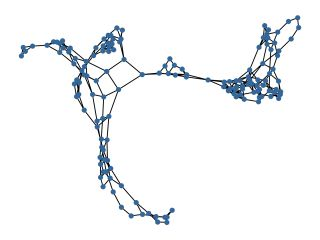
\includegraphics[scale=4]{protein.jpg}
\caption{Graf proteina}
\label{fig:protein}
\end{figure}
Nije odgovarala činjenica da je prikaz molekula proteina zapravo neusmjereni graf pa je matrica susjedstva čvorova simetrična, što je upola manje računskog posla od onog koji bi bio potreban za naš projekt jer se uzima samo donji trokut u izračunima. Cilj našeg projekta je dobiti usmjereni graf. U radu se spominje kako je moguće napraviti preinake matrice, izračunati i gornji trokut. Također, zbog specifične forme dataseta, prilagodba na vlastiti dataset bila bi mukotrpna. Od pristupa se odustalo jer su pronađeni oni koji više obećavaju i kojima je potrebno manje prilagodbe. 

\section{Latent Skill Embedding (Lentil)}
\subsection{Općenito o Lentil-u}
%izvještaj prvog tjedna
Pronađen je i istražen gotovo na samom početku prakse. Daljnjim istraživanjem pokazuje velik potencijal \citep{lentil}. Sažeto ga je moguće definirati kao sustav za personaliziranu preporuku nastavnih cjelina. Metoda je upravljana podacima, uči reprezentaciju sadržaja koja ne zahtijeva \textit{a priori} znanje preslikavanja \textit{content-to-concept}. Proširuje ideje \textit{sparse factor analysis} (SPARFA) i multidimenzionalne Item Response Theory.\newline
Model uči prikaz korisničkog znanja, kao i edukacijski sadržaj kako bi se prikazale preporuke, personalizirane upute o učenju. Probabilistički je model. Problem je formuliran kao regularizirani \textit{maximum-likelihood embedding} korisnika, nastavnih cjelina (lekcija) i procjena znanja (ispita) u zajednički semantički prostor (latentni prostor vještina) iz skupa podataka o prošlosti interakcije korisnik-sadržaj (\textit{access traces}). Nastavne cjeline i procjene znanja su moduli sadržaja. Fiksni su, a korisnici imaju putanje latentnim prostorom vještina. Stvara se multidimenzionalno okružje - studentsko znanje “leži” u kontinuiranom prostoru stanja, a preduvjeti lekcija moduliraju dobitke znanja lekcijskih modula. Ugradnja u taj prostor ne koristi simetrične udaljenosti komponenata, već se bilježi prirodni napredak težine procjene znanja i rasta korisničkog znanja.\newline
Korisnik je prikazan kao skup latentnih vještina, nastavna cjelina kao vektor dobitaka vještina i skupa preduvjeta, a procjena znanja kao skup potrebnih vještina. Korisniku se procjenjuje znanje nekog modula (ne zna ili zna, 0 ili 1), a vjerojatnost da će proći je veća ako korisnik ima visoku razinu vještine koja nadmašuje potrebne vještine za procjenu. Korisnik može poboljšati vještinu vremenom (koje je diskretizirano). Naglašava se da bi za poboljšanje vještine trebalo gledati korisničko predznanje (ovisno o predznanju podešavati težine u jednadžbi modela). 

\subsection{Ideje}
U radu je istražena i implementirana ideja određivanja slijeda lekcija pri praćenju znanja što se ispostavilo kao veoma primjenjivo na naš problem. Temelj eksperimenata s ovim modelom bila je vizualizacija slijeda zadataka. U kasnijoj etapi projekta, povratkom na ovaj obećavajući model, u originalni se kod implementiralo grupiranje zadataka kada su poznate pripadnosti koncepata i zadataka. Velika početna prednost modela je što koristi pronađeni Assistments dataset koji je prvi pronađen u sklopu projekta i koji služi kao glavni temelj za usporedbu. Razmišljalo se na koji način je prigodnom veličinom dataseta moguće osigurati dovoljnu varijabilnost puteva učenja. \newline
U originalnim .ipynb bilježnicama primijećene su mnoge instance korisničkih putanja koje dijele iste lekcijske module na početku i module procjene na kraju, ali se sastoje od različitih lekcija tijekom učenja → stvaraju se mjehurići, \textit{bubbles}, koji su zapravo eksperimentalni dokaz dobrih svojstava različitih pristupa učenju. Prikazani su na slici ~\ref{fig:bubbles}. Mjehurići se koriste za evaluaciju sposobnosti ugradnje preporuke slijeda lekcija koja vodi do uspješnog ostvarenja ciljeva učenja. Model logističke regresije s L2 regularizacijom korišten za procjenu vjerojatnosti da će korisnik slijediti preporučenu “granu” mjehurića. Unutar svakog mjehurića, korisnici koji su krenuli preporučenim putem spojeni su s najbližim susjedom iz grupe onih koji nisu slijedili preporučeni put prema razlici u \textit{propensity scoreu}.

\begin{figure}[!htb]
\centering
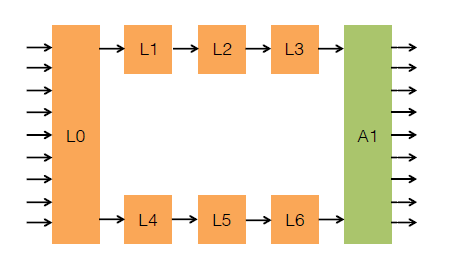
\includegraphics[scale=1]{bubbles.PNG}
\caption{Prikaz mjehurića, različitih putanja tijekom učenja \citep{lentil}}
\label{fig:bubbles}
\end{figure}

\subsection{Problemi i zadaci}
Kao početni potencijalni problem izvedbe modela pokazala se činjenica da su ocjene znanja modelirane na različitim osima grafičkih prikaza što za sobom povlači neovisnost lekcija i vještina, što ne mora u stvarnosti biti slučaj. Također, u prikazu putanja, u originalnim ispitnim podacima u radu vidljiva je pristranost korisničkih putanja jednoj vrsti temeljne, česte putanje zbog sličnosti pozadinskog znanja ispitanika.\newline
Isto tako, pronađena je greška u originalnom kodu; činjenica da se prijeđene putanje korisnika ne broje na odgovarajući način (iteriranje liste tupleova bezuspješno, uvijek 0).\newline
Pri početnom ostvarivanju vizualizacije slijeda zadataka kao problem je okarakterizirana činjenica da crta vektore (vidljivo na slici ~\ref{fig:lentil}), a ne pravi graf koji “povezuje” korisnike preko procjena ovisno o vještinama dobivenih nakon neke lekcije (više ukazuje na smjer potencijalnog puta, što isto donekle odgovara cilju projekta).\newline 

\begin{figure}[!htb]
\centering
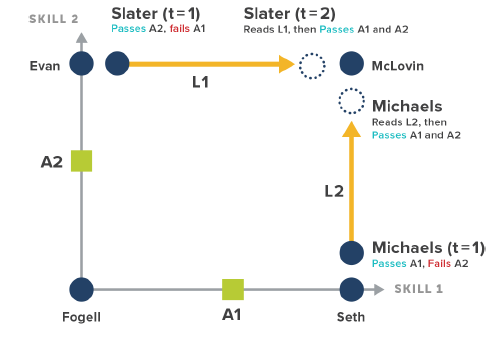
\includegraphics[scale=1]{lentil.PNG}
\caption{Grafički prikaz Lentil-a (korisnika, lekcija, testova i napretka ovisno o točnosti \citep{lentil}}
\label{fig:lentil}
\end{figure}
Izrađena je prilagodba na Google Colab, koja se pokazala izazovnijom od očekivanog zbog zastarjelosti originalnog koda i činjenice da je Google Colab službeno ukinuo podršku za Python 2.7 (iako je ipak i dalje moguće pokretati sadržaj).\newline
Nakon uspješne vizualizacije slijeda rješavanja zadataka Assistments dataseta, ideja je bila pokušati prilagoditi model našem "Biologija" datasetu. Potrebno je bilo riješiti problem prisutnosti varijabli trajanja i vremenskih koraka u originalnim funkcijama jer mi to ne gledamo i ne trebamo te spajati čvorove zadataka ovisno o pripadnosti pojedinom konceptu ili još bolje, spajati koncepte. 

\subsection{Rezultati}
Nakon početnog ispravljanja grešaka u kodu, dobiven je string koji označuje povezanosti čvorova dataseta na način da su strelicom povezani zadaci koje jedan korisnik rješava jedan za drugim prema pojavi u datasetu. Vizualizacija toga na cijelom datasetu generirala se preko 8 sati jer PyGraphviz, Pythonovo sučelje Graphviza (alata za crtanje grafova), ne iskorištava mogućnosti ubrazanja u Google Colabu. Odlučeno je prilagoditi i smanjiti dataset (uzeti prvih 200 redaka). Nakon toga uspješno je izvršena vizualizacija dvije vrste grafova koji prikazuju povezanost zadataka:
\begin{itemize}
\item graf tijeka (engl. \textit{flow grah}) - zadaci Assistment dataseta predstavljaju čvorove grafa koji se povezuju ovisno o korisničkom pristupu konkretnom problemu. Prikaz je vidljiv na slici ~\ref{fig:dot1}.
\item graf veza (engl. \textit{connection grah}) - čvorovi su i korisnici i zadaci kojima oni pristupaju. Prikaz je vidljiv na slikama ~\ref{fig:dot2} i ~\ref{fig:sfdp2}.
\begin{figure}[!htb]
\centering
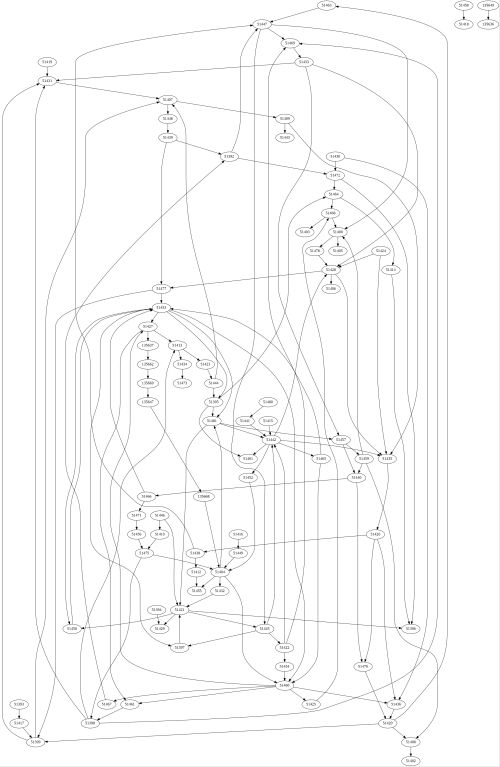
\includegraphics[scale=0.5]{dot1.jpg}
\caption{Originalni "dot" graf tijeka s podacima smanjenog Assistment dataseta}
\label{fig:dot1}
\end{figure}
\end{itemize}

\noindent Eksperimentiranjem s PyGraphvizom moguće je dobiti različite vizualne prikaze istog grafa (odnosno rasporede - dot, neato, twopi, circo, fdp, sfdp), pa je ovisno o namjeni moguće izabrati najprikladniji. Neki od prikaza vidljivi su na slikama ~\ref{fig:circo1} i ~\ref{fig:sfdp1}.

\begin{figure}[!htb]
\centering
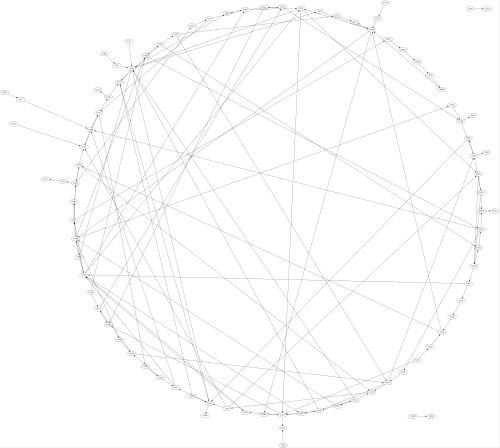
\includegraphics[scale=0.4]{circo1.jpg}
\caption{Originalni "circo" graf tijeka s podacima smanjenog Assistment dataseta}
\label{fig:circo1}
\end{figure}

\begin{figure}[!htb]
\centering
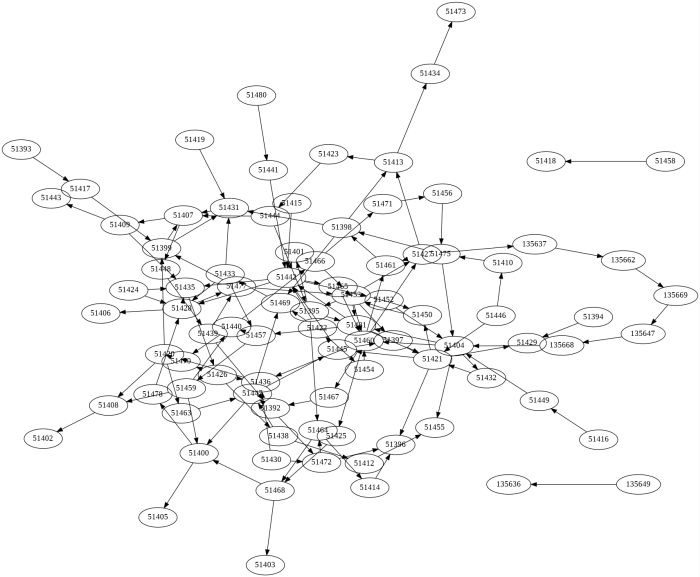
\includegraphics[scale=1.3]{sfdp1.jpg}
\caption{Originalni "sfdp" graf tijeka s podacima smanjenog Assistment dataseta}
\label{fig:sfdp1}
\end{figure}

\begin{figure}[!htb]
\centering
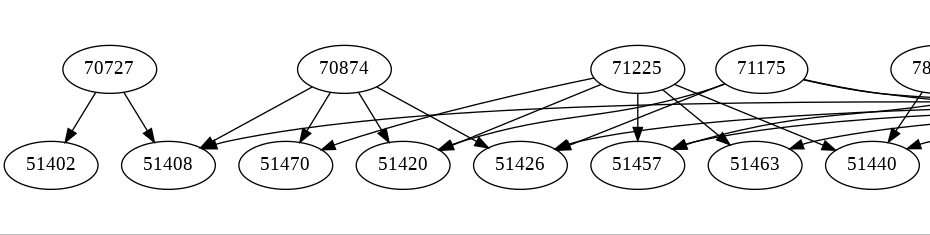
\includegraphics[scale=0.35]{dot2.png}
\caption{Originalni "dot" graf veza s podacima smanjenog Assistment dataseta}
\label{fig:dot2}
\end{figure}

\begin{figure}[H]
\centering
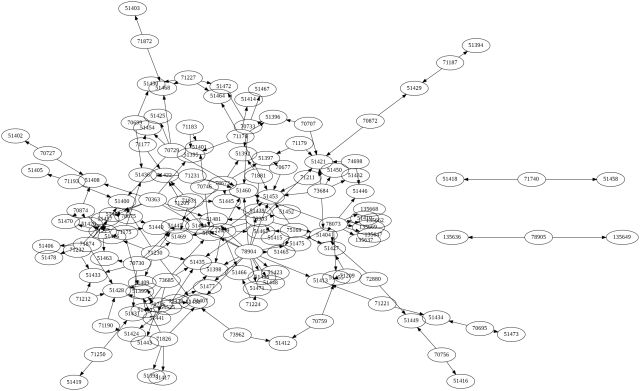
\includegraphics[scale=1.7]{sfdp2.jpg}
\caption{Originalni "sfdp" graf veza s podacima smanjenog Assistment dataseta}
\label{fig:sfdp2}
\end{figure}

\noindent Nakon ovakvog prikaza moguće je bilo zaključiti prednosti i nedostatke pojedine vrste prikaza.\newline
Graf veza mnogo je manje intuitivan i manje pregledan od grafa tijeka. Za daljnje eksperimentiranje, kao prikladniji graf uzet je graf tijeka zbog veće preglednosti i veće prilagođenosti našem problemu. No, iako je preglednost znatno bolja nego kod grafa veza, svejedno nije u potpunosti zadovoljen kriterij preglednosti. Zadaci različitih korisnika nisu obojeni različitim bojama, a ni pristup samim zadacima nije kronološki.\newline
Za intuitivniju vizualizaciju putanja dodane su oznake pojedinih korisnika između čvorova, što je vidljivo na slici ~\ref{fig:dot3}. Ideja je poboljšati dodavanjem različitih boja svakom korisniku. 

\begin{figure}[!htb]
\centering
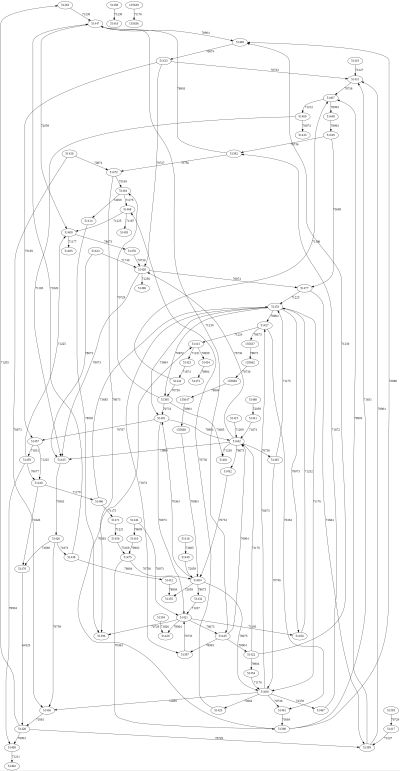
\includegraphics[scale=1.8]{dot3.jpg}
\caption{"dot" graf tijeka s podacima smanjenog Assistment dataseta uz dodane oznake korisnika}
\label{fig:dot3}
\end{figure}

\chapter{Clustering}
Početno se razmatralo na osnovu čega bismo u modelu preporuka mogli napraviti ostvarenje vizualizacije grupiranja (engl. \textit{clustering}) zadataka u koncepte ako nemamo označenu eksplicitnu pripadnost. Kao moguća ideje spominjao se redoslijed rješavanja, no zbog nerealnosti takve situacije najbrže je odbačena. Dodatno, moglo bi se gledati točnost pojedinih odgovora velikog broja ispitanika.
%-napravimo neku dodatnu varijablu mastery_score koja raste s točno riješenim zadatkom pa pratimo prema tome

\section{Latent Skill Embedding (Lentil)}

\noindent Nakon kratkotrajnog napuštanja Lentil modela zbog bavljenja modelima koji više obećavaju, napravljen je povratak u sklopu istraživanja za zadatak grupiranja zadataka ako nemamo eksplicitno definiranu pripadnost konceptima.\newline
Prvo je istražena mogućnost vizualnog grupiranja zadataka u okviru Lentil koda ako imamo pripadnost konceptima. Takva vizualizacija služila bi za usporedbu točnosti s modelom koji bismo osmislili. To je uspješno izvršeno. Dodan je stupac informacije o konceptima dataseta Assisstments u kod. Smanjenom datasetu za probu (20 pitanja) dodijeljene su različite oznake koncepata te je izvršeno grupiranje zadataka po konceptima izmjenom funkcije koja stvara graf tijeka manipulacijama s Pandasom (čvorovi su zadaci, na vezama oznake korisnika koje su ih riješile). Vizualizacija se nalazi na slici ~\ref{fig:clust1}. \pagebreak

\begin{figure}[!htb]
\centering
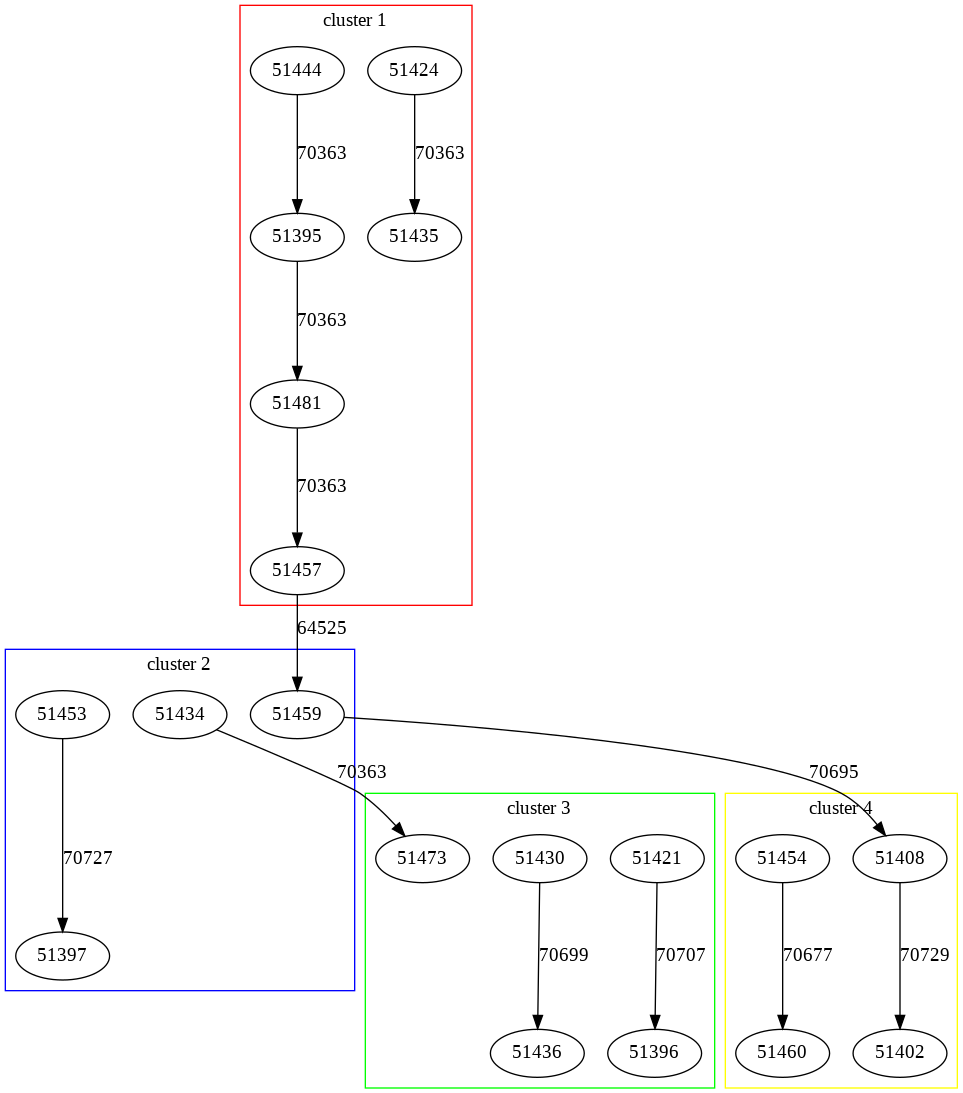
\includegraphics[scale=0.3]{clust1.png}
\caption{Grupiranje zadataka smanjenog Assistments dataseta prema pripadnosti konceptima}
\label{fig:clust1}
\end{figure}

\noindent Isti rezultat dobiven eksperimentom s drugačijim pristupom (izračunom matrice prijelaza između stanja (čvorova) Markovljevog modela). Grupiranje zadataka je identično kao na slici ~\ref{fig:clust1}, ali je prikaz manje interpretabilan jer u ovoj fazi ne prikazuje oznake korisnika. Vidljiv je na slici ~\ref{fig:clust2}.\newline 

\begin{figure}[!htb]
\centering
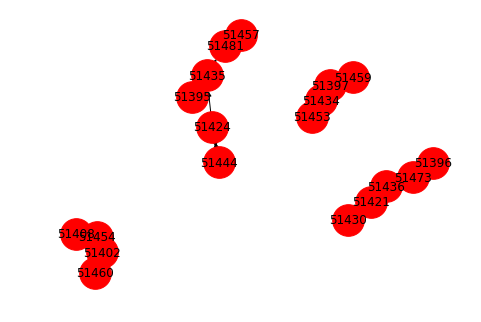
\includegraphics[scale=0.4]{clust2.png}
\caption{Grupiranje zadataka smanjenog Assistments dataseta prema pripadnosti konceptima izračunom matrice prijelaza}
\label{fig:clust2}
\end{figure}
\pagebreak

Konkretno, koristi se provjera različitosti pojedinih pitanja. Svaki zadatak teorijski je modeliran kao stanje Markovljevog procesa (diskretni stohastički proces je Markovljev proces ako vjerojatnost prijelaza u određenom diskretnom trenutku ovisi o stanjima u svim trenutcima prije). Stvara se matrica prijelaza između stanja (čvorova koji predstavljaju pitanja). Na osnovi takve matrice crta se graf. Kasnije se računa matrica vjerojatnosti prijelaza stanja pa stacionarna distribucija (vjerojatnosna distribucija koja se ne mijenja u Markovljevom lancu kako vrijeme prolazi). \newline
Ponovno čitanje rada \citep{lentil} inspiriralo je za ideju korištenja izračuna entropije za određivanje koncepata. Entropija se računa kao negativni skalarni produkt stacionarne distribucije i $Plog(P)$, gdje $P$ predstavlja matricu vjerojatnosti prijelaza među stanjima. Sama korist izračuna entropije još nije prikazana. Entropija inače predstavlja “porast informacije u podatcima”. Potencijalno, ideja je da, s obzirom da se računa za svaku matricu vjerojatnosti prijelaza, za svaku putanju različitih korisnika računati entropiju i utvrditi postoje li pravilnosti koje pomažu odrediti koncepte. 

\section{K-Medoids}
Kao odvojeni pristup, napravljena je skripta koja radi clustering pomoću algoritma K-Medoids.\newline
Kao vektor, odnosno element dataseta koji treba grupirati, uzeta je lista odgovora svih ispitanika na određeno pitanje (jedan element predstavlja jedno pitanje). Za metriku udaljenosti napravljena je funkcija koja gleda sumu razlika dva vektora (gleda se razlika između $x[i]$ i $y[i]$ za $i \in [0, broj ispitanika-1]$). Može se uzeti i kvadratni korijen te sume.\newline
Definirana je i funkcija koja računa grešku kao sumu elemenata koji nisu dobro grupirani. Uzeto je da je “prava” klasa ona kojoj pripada najviše elemenata iz tog koncepta, a oni koji nisu u njoj, pridodani su ukupnoj sumi greške. 
Grupiranje se radi na standardiziranim i nestandardiziranim podacima i za obje verzije računaju se \textit{rand index}, \textit{adjusted rand index}, NMI vrijednost (\textit{normalized mutual information}) te ranije spomenuta funkcija koja računa broj krivo grupiranih primjera.\newline
Napravljena je i funkcija koja metodom lakta određuje idealan broj klasa, u slučaju da on nije otprije poznat.
\newline
\newline
Za različite datasetove skripta pokazuje funkcionalnost na različite načine.\newline
Biologija dataset:\newline
Za sad je algoritam isproban samo na datasetu Biologija (84 odgovora) jer je Assistments malo prevelik, ali sljedeći korak je testiranje i na Assistments.\newline
Dataset ima 30 pitanja, znači imamo 30 ulaznih vektora. Algoritam je isproban na standandiziranim i nestandardiziranim podacima, te daje nešto malo bolje rezultate na nestandandiziranim, ali to može biti i do dataseta. 
Rand index na nestandardiziranim podacima je 0.83, a adjusted rand index 0.41, za što kažu da spada u “srednje dobar rezultat”. NMI vrijednost je oko 0.58, a minimum koji se dobiva funkcijom za sumu greške jest 9 (od ukupno 30 pitanja). Lošiji rezultati mogu biti i do dataseta Biologija koji je svakako daleko od idealnog, jer ni koncepti nisu dobro definirani (npr. ispitanik možda ne zna živčanu stanicu, ali je čuo odgovor na par pitanja iz psihologije). 
Korištenjem metode lakta za određivanje broja klasa dobije se 6 klasa, što je vidljivo na slici ~\ref{fig:medoids_bio}, dok je pravi broj klasa 5.

\begin{figure}[!htb]
\centering
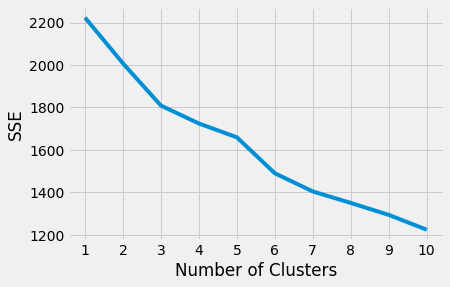
\includegraphics[scale=0.5]{medoids_bio.png}
\caption{Prikaz određivanja klasa iz Biologija dataseta korištenjem metode lakta}
\label{fig:medoids_bio}
\end{figure}

Assistments dataset:\newline
Testiranje na Assistments u početku je okarakterizirano kao nemoguće jer K-Medoids algoritam zahtijeva da su svi vektori iste dimenzionalnosti odnosno da su svi ispitanici odgovorili na sva pitanja. To u Assistments nije zadovoljeno. Eventualno se može probati s nekakvom redukcijom dimenzionalnosti vektora (npr. \textit{principal component analysis}, međutim budući da ima pitanja na koja je samo jedan student odgovorio, na kraju bismo trebali završiti s dimenzionalnošću 1 (što je puno premalo da bi obuhvaćalo potrebne informacije).\newline
U nastavku rada na ovom pristupu, napravljena je prilagodba za učitavanje smanjenog Assistments dataseta (20 pitanja). No, početna pretpostavka da testiranje s Assistemntsom neće biti moguće pokazala se ispravnom. Isprobana je metoda grupiranja slična K-Medoids, K-Means, ali nije pokazala željenu funkcionalnost.

\section{Ostatak istraživanja}
Mnogi radovi pokazali su se u cjelovitosti ne toliko relevantnima da bismo ih mogli u potpunosti primijeniti na naš problem, ali su predstavili mnoge iskoristive koncepte i algoritme vrijedne spomena.\newline
\newline
U radu \citep{its} spominje se da je razumijevanje krajnjeg cilja svakog studenta praćeno pomoću posebne varijable mastery\_score koja se osvježava svaki puta kada se vrši procjena studentovog znanja. \newline
Spominje se da identificiraju i vizualiziraju grupe povezanih koncepata. Točnije, \textit{spreading algorithm} pronalazi uzorak u povezanosti koncepata i dokumenata te dokumenata i koncepata. Analizirana je struktura \textit{spreading algorithma} \citep{spreading}.\newline
Problem je što je potrebna neka vrsta reference, ekspertno određenog početnog grafa koji će se evaluirati tim algoritmom.\newline
\newline
U radu \citep{dhkt} predstavljene su hijerarhijske veze pitanja i koncepata modelirane pomoću hinge loss skalarnog produkta ugrađenih koncepata i pitanja. Problem: povezanost koncepata i pitanja određena ekspertima i zapisana u matrici ugradnje, a eksperte želimo izbjeći. Korišten je t-distributed stochastic neighbor embedding (tSNE) algoritam.
tSNE je algoritam strojnog učenja za vizualizaciju; nelinearna tehnika za redukciju dimenzionalnosti. Koristi se za ugradnju visokodimenzionalnih podataka za vizualizaciju u niskodimenzionalni prostor (2 ili 3 dimenzije). Slični objekti su s visokom vjerojatnosti modelirani točkama koje su blizu u prostoru, a različiti objekti udaljenim točkama \citep{tdsne}.
Problem: velika osjetljivost algoritma na promjenu parametara.\newline
\newline
Rad \citep{conc_rel} primarno radi poveznicu između samih koncepata, ali i između koncepata i objekata učenja (zadataka, primjera, itd.) uz pretpostavke da je broj objekata učenja poznat. Glavni problem i razlog napuštanja ovakvog modela je što se \textit{preprocessing} objekata učenja radi pomoću \textit{text-mininga}. Isto tako, rad pretpostavlja da je netko nekad označio povezanost koncepata i objekata učenja pa da može koristiti tu referencu. Nad tom referencom oblikuje se tzv. \textit{contextual network} koja sadrži više vrsta čvorova. Za izračunavanje sličnosti koncepata koriste se dva načina: već spomenuti \textit{spreading activation algorithm} i \textit{PageRank with Priors}.\textit{ PageRank with Priors} koristi se kao kvantitativna mjera sličnosti čvorova prema nekom drugom čvoru. Čestu primjenu ima u sustavima kategorizacije.
U konkretnom primjeru, propagiraju se stvarne karakteristike modela domene znanja u eksplicitne veze među konceptima.\newline
\newline
U radu \citep{trans} veoma je izraženo shvaćenje da mnogi radovi poistovjećuju koncepte i zadatke i to pojednostavljenje uzrokuje probleme.\newline
Prepoznaju da grafovi znanja ciljaju da predstave znanje u obliku grafova tripleta; triju činjenica - (početni entitet, veza, završni entitet).\newline
Razlikuju povezanost koncepta i zadataka, koncepata međusobno te zadataka međusobno. Ovisno o vrsti povezanosti, koriste različite funkcije gubitka.\newline
Koncepte enkodiraju kao sfere, a zadatke kao vektore u istom semantičkom prostoru.\newline
Metoda je evaluirana pomoću predikcije veza i klasifikacije tripleta. Potonja ocjenjuje točnost tripleta.
Predikcija veza predviđa početni ili završni entitet iz tripleta, ovisno koji nedostaje. Algoritmu je potrebno dati rangirane preporuke zadataka, ne samo najbolji rezultat.
Sve mogućnosti se rangiraju kao moguće upopunjavanje traženog praznog mjesta prema udaljenosti u određenoj funkciji gubitka. Za evaluaciju koriste se dvije mjere:
\begin{enumerate}
\item srednja recipročna mjera svih točnih instanci (MRR) i
\item razmjer točnih zadataka koji rangiraju ne više od N (Hits@N).
\end{enumerate}
Glavni problem, kao i u većini istraženih metoda: znaju koliko je koncepata.\newline
\newline
Rad \citep{hgkt} slične vježbe grupira u koncepte naziva “problem schemas”. Koristi se hierarchical graph neural network. Konkretno, ovdje je mreža dvoslojna: donji je sloj zadataka (svaki čvor je jedan zadatak), gornji je sloj problemskih shema. Povezanost zadataka i problemskih shema modelira se \textit{assignment matrixom} koji se dobije pomoću \textit{hierarchical clustering analysis (HCA)}. HCA je metoda analize grupiranja bez nadzora korištenjem aglomerativnih ili divizivnih strategija za izgradnju hijerarhije grupa.
Za konstrukciju hijerarhijskog grafa zadataka spominje se iskorištavanje semantičke informacije zadataka i shema, ali kasnije se  spominje treniranje mreže samo pomoću HCA pa je i to jedan od pristupa koji valja detaljnije istražiti.\newline
\newline
Istražen je i alat Ampligraph \citep{ampl1, ampl2}. Površna analiza definirala ga je kao dosta moćan alat. Funkcionalnosti obuhvaćaju stvaranje grafa znanja, treniranje ugradbenog modela na tripletima, evaluaciju modela, vizualno grupiranje pojmova.
Problem: s obzirom da koristi triplete (subjekt, predikat, objekt), potrebno je poznavati povezanost pitanja.\newline
\newline
Daljnja proučavanja vratila su nas na rad s početka, Deep Knowledge Tracing (DKT), \citep{dkt}. U njemu je spomenuto kako se DKT model može koristiti za zadatke otkrivanja latentne strukture ili koncepata u podacima. Problemu je pristupljeno na način da se utjecaj $J_{ij}$ dodijeli svakom usmjerenom paru zadataka $i$ i $j$, gdje je $y(i | j)$ vjerojatnost točnosti koju RNN dodjeljuje zadatku $j$ ako je učenik u prethodnom koraku točno odgovorio na zadatak $i$. Opisano je vidljivo u jednadžbi ~\ref{eq:dkt}.
\begin{equation}
J_{i j}=\frac{y(j \mid i)}{\sum_{k} y(j \mid k)}\label{eq:dkt}
\end{equation}
\newline
Kao dodatni pristup prepoznat je i rad povezan s kasnije detaljno opisanim ExRec-om \citep{exrec}, Dynamic Key-Value Memory Network Knowledge Tracing (DKVMN) \citep{dkvmn}. U radu je spomenuto kako se bave otkrivanjem uzoraka (koncepata) zadataka pomoću korelacijskih težina. Korelacijske težine između zadataka i koncepata impliciraju snagu njihove povezanosti. Nije potrebno otkiriti ovisnosti među zadacima i onda definirati prag za grupiranje, kako je to obično u povezanim radovima. Svaki zadatak povezuje se s jednim konceptom prema najvećoj vrijednosti korelacijske težine. Spominje se i korištenje već spomenutog t-SNE algoritmna \citep{tdsne} za prikaz grafa projiciranjem multidimenzionalnih korelacijskih težina u 2D točke. Problem ovog pristupa je što nije jasno definirano kako stvaraju korelacijske težine. 
\chapter{Literatura}
\renewcommand{\bibsection}{}
\begin{thebibliography}{9}
	
	\bibitem[1]{ct1} Knewton, \url{https://www.knewton.com/blog/mastery/what-are-knewtons-knowledge-graphs/}
	\bibitem[2]{ct2} Deep Knowledge Tracing, \url{ http://papers.nips.cc/paper/5654-deep-knowledge-tracing.pdf}
	\bibitem[3]{ct3} KnowEdu, \url{ https://ieeexplore.ieee.org/stamp/stamp.jsp?tp=&arnumber=8362657}
	\bibitem[4]{ct4} Back to the basics: Bayesian extensions of IRT outperform
	neural networks for proficiency estimation, \url{https://arxiv.org/pdf/1604.02336.pdf}
	\bibitem[5]{ct5} Addressing Two Problems in Deep Knowledge Tracing via
	Prediction-Consistent Regularization, \url{https://arxiv.org/pdf/1806.02180}
	\bibitem[6]{ct6} Latent Skill Embedding (Lentil), \url{https://arxiv.org/pdf/1602.07029.pdf}
	\bibitem[7]{ct7} \url{https://www.analyticsvidhya.com/blog/2019/10/how-to-build-knowledge-graph-text-using-spacy/}
	\bibitem[8]{ct8} K12EduKG, \url{https://aic-fe.bnu.edu.cn/docs/20181205101832069569.pdf}
	\bibitem[9]{ct9} Deep Generative Models, \url{https://arxiv.org/abs/1803.03324}
	\bibitem[10]{ct10} \url{https://eigenfoo.xyz/deep-autoregressive-models/}
	\bibitem[11]{c11} Graph Recurrent Attention Networks, \url{https://arxiv.org/abs/1910.00760}
	\bibitem[12]{c12} Latent Skill Embedding (Lentil), \url{https://arxiv.org/pdf/1602.07029.pdf}
	\bibitem[13]{c13} \url{http://math.ubbcluj.ro/~tradu/TI/coverch4_article.pdf}
	\bibitem[14]{ct14} \url{https://www.slideshare.net/bamparopoulos/entropy-based-measures-for-graphs}
	\bibitem[15]{ct15} \url{https://www.educationaldatamining.org/EDM2015/proceedings/short360-363.pdf}
	\bibitem[16]{ct16} \url{https://www.researchgate.net/publication/333828640_INTERACTIVE_LEARNING_IN_A_CONVERSATIONAL_INTELLIGENT_TUTORING_SYSTEM_USING_STUDENT_FEEDBACK_CONCEPT_GROUPING_AND_TEXT_LINKING}
	\bibitem[17]{ct17} \url{https://en.wikipedia.org/wiki/Spreading_activation}
	\bibitem[18]{ct18} Deep Hierarchical Knowledge Tracing, \url{http://www.personal.psu.edu/ffm5105/files/2019/edm19.pdf}
	\bibitem[19]{ct19} \url{https://en.wikipedia.org/wiki/T-distributed_stochastic_neighbor_embedding}
	\bibitem[20]{ct20} Automatic Concept Relationships Discovery for an Adaptive E-course, \url{https://www.educationaldatamining.org/EDM2009/uploads/proceedings/simko.pdf}
	\bibitem[21]{ct21} Differentiating Concepts and Instances for Knowledge Graph Embedding, \url{https://www.aclweb.org/anthology/D18-1222/}
	\bibitem[22]{ct22} HGKT : Introducing Problem Schema with Hierarchical Exercise Graph for Knowledge Tracing, \url{https://arxiv.org/pdf/2006.16915v2.pdf}
	\bibitem[23]{ct23} Ampligraph, \url{https://docs.ampligraph.org/en/1.3.1/}
	\bibitem[24]{ct124} \url{https://github.com/Accenture/AmpliGraph/blob/master/docs/tutorials/ClusteringAndClassificationWithEmbeddings.ipynb}
	
\end{thebibliography}
\end{document}}